% ============================================================
% Motion-borne geometry — Quantum (quantum-journal.org) build,
% quantumarticle class (venue retargeted from SciPost 2026-08-14:
% institutional-email registration gate). quantumarticle loads
% hyperref and sets geometry itself. Canonical paper source.
% ============================================================
\RequirePackage[2023-06-01]{latexrelease} % quantumarticle v6.1 era
\documentclass[a4paper,11pt,noarxiv]{quantumarticle}
\usepackage{amsmath,amssymb}
\usepackage{graphicx}
\usepackage{booktabs}
\usepackage{array}
\usepackage{xcolor}
\definecolor{linkink}{HTML}{1c3f77}
\usepackage{hyperref}
\hypersetup{colorlinks=true,linkcolor=linkink,citecolor=linkink,
urlcolor=linkink}
\graphicspath{{../figures/}}
\newcommand{\ephi}{\varepsilon_\Phi}
\newcommand{\logr}{\log\rho}

\title{Does an emergent information metric need its dynamics? A
preregistered test in finite spin chains}
\author{Oleg Roshka}
\affiliation{Independent Researcher \textnormal{--}
\href{https://orcid.org/0009-0009-3075-9417}{ORCID
0009-0009-3075-9417}}
\date{\today}

\begin{document}
\maketitle

\begin{abstract}
Is a stable emergent structure merely \emph{instantiated} by its
substrate --- some motionless configuration would carry the same
structure --- or \emph{actively maintained} by the substrate's
dynamics? We turn this question into an operational test and apply it,
in a registered-study design, to the mutual-information-graph metric of
finite spin chains across fixed-point, quasiperiodic, chaotic,
metastable, localized, and driven (kicked-Ising, DTC-like) dynamics.
The test has three probes: null-silent witnesses of state motion
beneath the metric, a coherence-removal response, and an explicit
search for a stationary state carrying the same time-averaged metric.
Three results survive our own audits and an external pre-submission
review. First, time averaging and metric construction do not commute:
the diagonal ensemble, whose two-site reduced density matrices are
exactly the time averages, misses the time-averaged metric by
43--90\%, because mutual information is nonlinear in the state.
Second, the cost of repairing this mismatch is class-resolved and
size-robust: simple thermal-window ensembles reproduce chaotic-class
metrics almost exactly (miss $\sim 0.04$, consistent with eigenstate
thermalization), while the quasiperiodic time-averaged metric admits
no smooth-of-$H$ stationary reproduction (miss $\sim 0.32$, 0/80 runs)
and is reached only by fine-tuned population vectors whose parameter
count scales with Hilbert-space dimension --- an unrestricted
optimization matches it, so the discriminator is the \emph{description
complexity} of the cheapest motionless impostor, not its existence.
Third, weak dephasing \emph{pins} the moving quasiperiodic metric to
its time average (negative log drift ratio, stable over two decades of
noise rate) while destabilizing chaotic-class metrics --- the same
class is extremal on both instruments. The study record --- committed
seed manifests, a dated amendment log, five caught-and-corrected
failure modes (one prompted by external review), and all code and data
--- is public, and the corrections are reported as results.
\end{abstract}

\section{Introduction}\label{sec:intro}

A stable emergent structure can stand in two different relations to the
substrate that carries it. It can be \emph{merely instantiated}: some
motionless configuration of the substrate would carry the same
structure, and the observed dynamics is incidental to it. Or it can be
\emph{actively maintained}: the structure exists only because the
substrate moves, and no frozen configuration reproduces it. The
distinction is easy to state and surprisingly hard to test --- most
diagnostics of ``underlying dynamics'' do not actually certify that
anything is moving, and most claims of ``the dynamics sustains the
structure'' are never confronted with a serious search for a motionless
impostor.

This paper builds that test and runs it, in the most controlled setting
we could construct: finite spin chains, where the emergent structure is
the mutual-information-graph metric of
Refs.~\cite{SRC049,SRC060,SRC061} --- pairwise mutual information
converted to link weights and shortest-path distances on a posited site
factorization --- and the substrate dynamics ranges over fixed-point,
quasiperiodic, chaotic, metastable, localized, and driven
(kicked-Ising, DTC-like \cite{SRC043,SRC044,SRC054}) classes. Prior work on
such information-metric structures has been static: ground-state
network robustness under projective attacks \cite{SRC060}, metricity as
a phase diagnostic \cite{SRC061}. Our object is the \emph{time
dependence} of the structure over a moving state, and its need --- or
lack of need --- for that motion.

The test has three probes. A \emph{witness battery} certifies that the
state moves while the metric does not, under a requirement we treat as
non-negotiable: a witness of motion must vanish identically on a frozen
state. A \emph{coherence-removal response} measures what happens to the
metric when the state is projected onto its motionless diagonal
ensemble. And a \emph{motionless-comparator search} optimizes
explicitly over stationary states for one that carries the same
time-averaged metric. The study is a registered design --- every
metric, threshold, and analysis rule fixed before code was written,
every run seeded from committed manifests, every post-hoc change a
dated amendment (Appendix~\ref{app:log}) --- because a study of this
shape has one dominant failure mode, self-deception through flexible
metric choice, and we preferred to make our mistakes in public.

The mistakes were made, caught, and are reported as results. Five
times, a correction mechanism fired: a registered class certificate
was mis-specified (Poisson statistics for a free chain); the
out-of-time-order correlator, which we had registered as a witness of
state motion, fired on a frozen ground state --- the null test
correctly classifying it as an operator-spreading diagnostic
\cite{SRC064} rather than a state-motion witness; an early robustness
comparison was exposed by our adversarial re-analysis as a
floored-denominator artifact; a narrow first version of the comparator
search over-claimed unmatchability for two classes that a hardened
search then matched; and an external pre-submission review prompted an
unrestricted comparator optimization that overturned our remaining
existential claim. What survives this gauntlet is correspondingly
compact:
\begin{enumerate}
\item \textbf{An operational test} of instantiated-vs-maintained
  emergent structure (null-silent witnesses, coherence removal,
  motionless-comparator search), portable to any system with a
  computable structural functional.
\item \textbf{A non-commutation result.} Time averaging and metric
  construction do not commute: the diagonal ensemble --- the
  motionless state whose two-site reduced density matrices are exactly
  the time averages --- misses the time-averaged metric by 43--90\%.
\item \textbf{A complexity-resolved matching spectrum.} Repairing the
  mismatch is possible for every class, but at class-resolved cost:
  chaotic-class metrics are matched by simple thermal windows
  ($\sim$3 parameters, miss $\sim 0.04$); the quasiperiodic metric
  admits no smooth-of-$H$ reproduction (0/80 runs at $\sim 0.32$) and
  yields only to unrestricted, dimension-scaling population
  optimization. The class discriminator is the description complexity
  of the cheapest motionless impostor.
\item \textbf{A sign structure.} Weak dephasing \emph{stabilizes} the
  moving metrics of coherence-carried classes (negative log drift
  ratio, flat over two decades of noise rate) while destabilizing
  chaotic-class metrics --- the class that is hardest to match is the
  one noise defends. The mechanism is standard decoherence damping
  \cite{SRC059}; the class-resolved geometric reading appears, within
  the scope of our survey \cite{SRC060,SRC061,SRC062,SRC063}, to be
  unreported.
\item \textbf{A methods record.} The null-silence filter, the
  registered/amended/pre-committed staging of sharp statistical
  criteria with a measured seed-lottery episode, and the complete
  dated amendment log as Appendix~\ref{app:log}.
\end{enumerate}
The driven track adds an instructive case study: the DTC-like regime's
metric survives removal of its drive unchanged --- localization, not
the subharmonic motion, holds it (Sec.~\ref{sec:driven}).

\paragraph{What this paper does not claim.} The metric is an
information-theoretic construct on a posited factorization; its
factorization dependence is measured (Sec.~\ref{sec:scope}) and it is
not spacetime geometry --- no claim here touches gravity or holography.
No mechanism is claimed as new physics. No assumption is made that
information is ontologically primitive. All dynamics is stated against
an external laboratory clock. We make no priority claims about
preregistration in computational physics; the artifact is offered, not
its firstness. The model family is small ($N \leq 14$) and the
conclusions are in-model.

Section~\ref{sec:setup} defines the family, functional, witnesses, and
protocol; Secs.~\ref{sec:existence}--\ref{sec:driven} report results;
Sec.~\ref{sec:scope} states the scope walls; Sec.~\ref{sec:discussion}
discusses what the test opens up.

\section{Models, functional, witnesses, and protocol}\label{sec:setup}

\subsection{Model family}\label{sec:family}

All models are open chains of $N$ qubits with $\hbar = 1$ and the
nearest-neighbour coupling setting the unit of energy and time. Every
dynamical statement below is made with respect to an external
laboratory clock; the drive of the Floquet family defines a second,
stroboscopic clock derived from it. Nothing in this study bears on the
question of clocks internal to a system, which we regard as out of
scope.

We use three tracks. Track~A collects four closed-system classes chosen
to span the qualitative types of quantum motion
(Table~\ref{tab:classes}).

\begin{table*}[t]
\centering\small
\begin{tabular}{@{}p{2.1cm}p{4.6cm}p{4.2cm}p{3.2cm}@{}}
\toprule
class & Hamiltonian & initial ensemble & class certificate \\
\midrule
(i) fixed point & transverse-field Ising, $H=-\sum_i
\sigma^z_i\sigma^z_{i+1} - g\sum_i\sigma^x_i$, $g=1.5$ & ground state
(single deterministic run) & gapped, nondegenerate \\
(ii) quasiperiodic & XX chain,
$H=\tfrac12\sum_i(\sigma^x_i\sigma^x_{i+1}+\sigma^y_i\sigma^y_{i+1})$ &
20 superpositions of 3 single-magnon modes, pairwise-incommensurate
Bohr gaps & free-spectrum reconstruction $<10^{-8}$ \\
(iii) chaotic & mixed-field Ising, $(h_x,h_z)=(0.9045,0.8090)$ & 20
Haar-random product states & $\langle r\rangle =
0.529\text{--}0.542 \in [0.51,0.55]$ \\
(iv) metastable & ferromagnetic Ising, $g=0.05$, dressings $\delta g_i
\in [-0.01,0.01]$ & $\lvert\uparrow\cdots\uparrow\rangle$, 20 dressings
& quasi-degenerate doublet \\
\bottomrule
\end{tabular}
\caption{Track-A classes. Certificates are preregistered sanity checks,
run at every system size used before any confirmatory analysis.}
\label{tab:classes}
\end{table*}

Track~C reuses the chaotic and quasiperiodic Hamiltonians as
``scrambling'' and ``integrable'' regimes with N\'eel-anchored
product-state ensembles, and adds a localized regime (XXZ with random
fields, $\Delta=1$, $W=8$; 20--40 disorder realizations; $\langle
r\rangle = 0.38$--$0.40 \in [0.36,0.42]$). Track~B is a kicked-Ising
discrete time crystal modeled on the established protocol
\cite{SRC043,SRC044}: an imperfect global $\pi$-flip ($\varepsilon$ the
imperfection) alternating with disordered Ising interactions, 20
disorder realizations $\times$ 5 initial product states, with two
comparator regimes --- no interactions (r1) and no disorder (r2).

The class certificates are \emph{preregistered sanity checks}. One
failed as originally registered: we specified a Poisson
level-statistics window for the integrable class, which is a heuristic
for generic integrable models and is inapplicable to a free chain whose
many-body spectrum is exactly the subset-sums of its single-particle
spectrum. The replacement certificate --- reconstruction of the
many-body spectrum from single-particle energies to $10^{-8}$ --- is
strictly stronger, and the mis-specification plus its dated repair are
part of the study record (Appendix~\ref{app:log}). A second certificate
finding: the quasiperiodic incommensurability requirement is
\emph{exhaustively unsatisfiable} at $N=8$ (0 of 56 magnon triples
pass), which fixed the usable size range $(10, 12)$ for class
comparisons.

\subsection{The information metric and its stationarity}\label{sec:metric}

From the state (pure or mixed) we compute all one- and two-site reduced
density matrices, the pairwise mutual information $I_{ij} = S_i + S_j -
S_{ij}$, and normalize $x_{ij} = I_{ij}/(2\ln 2)$. Following the
emergent-metric construction of Ref.~\cite{SRC049}, link weights are
$w_{ij} = -\ln x_{ij}$, regularized by a floor $x_{\min}=10^{-6}$, and
the \emph{metric} $D(t)$ is the matrix of weighted shortest-path
distances on the complete graph over sites
(Fig.~\ref{fig:pipeline}). We emphasize the scope of the word
``metric'' here: $D$ is the metric structure of the mutual-information
graph on a \emph{posited} site factorization. It is not a claim about
spacetime, and its dependence on the factorization is measured, not
assumed away (Sec.~\ref{sec:scope}).

\begin{figure*}[t]
\centering
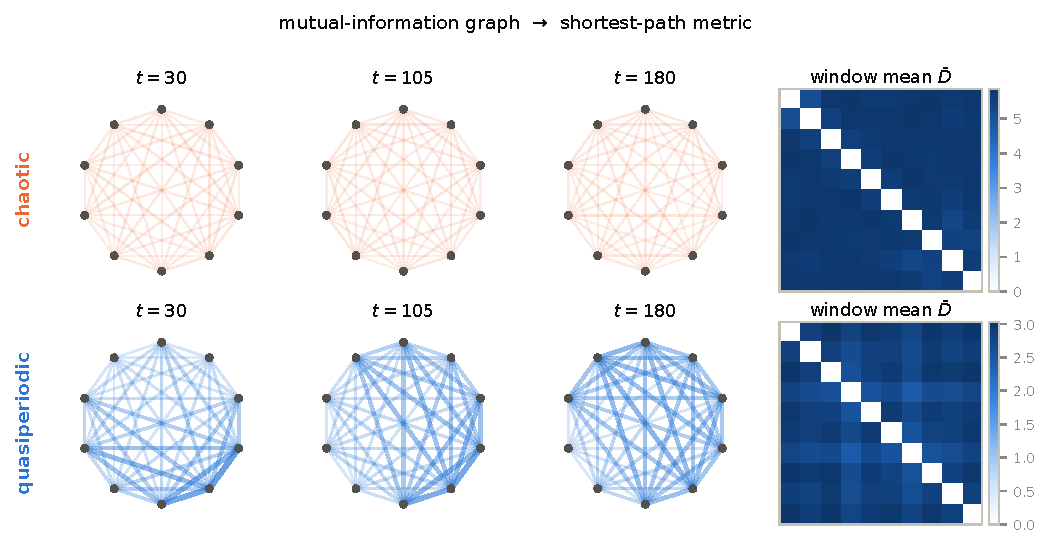
\includegraphics[width=\textwidth]{fig1_pipeline.pdf}
\caption{The pipeline, on real data (representative $N=10$ runs).
Nodes are sites; edge weight is pairwise mutual information; the
metric $D$ is the shortest-path distance matrix. Top: a chaotic-class
state --- the graph barely changes across the analysis window (its
weak, near-uniform mutual information yields the large, static
distances of the window mean $\bar D$). Bottom: a quasiperiodic
state --- the graph visibly rearranges as the incommensurate magnon
beats evolve.}
\label{fig:pipeline}
\end{figure*}

Stationarity is judged on the window $\mathcal{W} = [20, 200]$ (units
of inverse coupling; stroboscopic periods for Track~B), sampled every
$\Delta t = 0.5$: with $\bar D$ the window mean and $\delta\Phi(t) =
\lVert D(t)-\bar D\rVert_F / \lVert\bar D\rVert_F$, the metric is
stationary iff $\max_{t\in\mathcal W}\delta\Phi(t) < \ephi = 0.25$. The
threshold was set by a preregistered calibration pilot that measured
the construction's finite-size fluctuation floor (the originally
registered $0.05$ sat below the noise floor of every dynamical class
--- an instrument artifact the pilot existed to catch;
Appendix~\ref{app:log}, Amendment~3). A cap diagnostic --- the same
drift restricted to above-floor links --- is reported alongside every
verdict to expose any cap dominance; none of the verdicts below is
cap-dominated.

\subsection{Witnesses and the null-silence requirement}\label{sec:witnessdef}

The claim ``the metric is stationary while the state moves'' is only as
good as the certificate of motion. We require every \emph{witness of
motion} to satisfy a null-silence condition: \textbf{it must vanish
identically on a frozen state.} The null comparator is class~(i) ---
an eigenstate, whose evolution is a global phase --- and the
preregistered rule is that any witness which fires on the null is
discarded as a witness, whatever its other virtues.

The battery: (W1) the participation ratio $\mathrm{PR}_A$ of the binned
Bohr spectral measure
\begin{equation}
A(\omega) \;=\; \sum_{m,n}|c_m|^2\,|c_n|^2\;
\delta\!\big(\omega - |E_m-E_n|\big),
\end{equation}
equal to 1 exactly on the null; (W2) the recurrence
distance $d(t) = 1-|\langle\psi(t_0)|\psi(t)\rangle|^2$, identically
zero on the null, summarized by its window mean; (W4) the off-diagonal
energy coherence $\Xi = \sum_{E_m\neq E_n}|\rho_{mn}|^2$, computed over
energy-\emph{distinct} pairs so that coherence within a degenerate
level --- which does not move --- does not fire it; and, for Track~B,
(W5) the subharmonic Fourier weight of the stroboscopic magnetization
at half the drive frequency, with its rigidity curve $h_{\rm
sub}(\varepsilon)$. All are invariant under global phase and basis
relabelings in the senses catalogued in Appendix~\ref{app:battery}.

We also registered (W3) an out-of-time-order correlator,
$C(r,t)=\tfrac12\langle|[\sigma^z_{i_0+r}(t),\sigma^z_{i_0}]|^2\rangle$,
with saturation value and arrival time as statistics. The null test
disqualified it for \emph{our specific purpose} --- measured, not
argued: on the frozen fixed point it rises to $C\approx 1.11$ by
$t=1.5$. This is not a defect of the OTOC. OTOCs are understood in the
primary literature as diagnostics of Heisenberg-operator spreading
\cite{SRC064}, which a gapped ground state supports, and firing on an
eigenstate is expected behaviour for such an object. The point the
null test makes is narrower and, we think, worth making: an
operator-spreading diagnostic is not a witness of \emph{state} motion,
and the two roles are easy to blur when ``dynamics'' is used
informally. Under the registered rule its statistics were removed from
the class-separation criterion, with consequences reported in
Sec.~\ref{sec:witness}; it remains in our outputs in its proper role.

\subsection{Comparators and perturbation protocols}\label{sec:protocols}

Three controls give the sustained-by test its content. The
\emph{diagonal ensemble} $\bar\rho = \sum_n |c_n|^2
|n\rangle\langle n|$ is the canonical motionless partner of a run:
exactly stationary, with the same time-averaged two-site reduced
density matrices. We registered it as ``matched to the time-averaged
metric by construction'' --- which is false, and measurably so: mutual
information is nonlinear in the (correctly time-averaged) reduced
density matrices, and $\Phi[\bar\rho]$ sits 43--90\% away from $\bar D$
depending on class. The corrected comparator methodology --- an
explicit optimization over stationary states --- is described with its
results in Sec.~\ref{sec:comparator}. The \emph{coherence-removal test}
projects the state onto its diagonal ensemble mid-window (energy-basis
dephasing; populations are conserved, so the result is exactly
$\bar\rho$) and asks whether the metric's behaviour changes. We
emphasize what this operation is not: it is not switching the
Hamiltonian off --- setting $H=0$ would freeze the current state and
its metric in place --- it removes energy-basis coherence, i.e.\ the
motion, while keeping the time-averaged local structure. The driven
track uses a genuinely different operation, \emph{drive removal}
(Sec.~\ref{sec:driven}). And three \emph{perturbation
protocols} --- a local Hamiltonian quench $\lambda\sigma^z$, a local
dephasing channel of rate $\gamma$, and the loss of two non-adjacent
sites --- probe robustness through the scale-free log drift ratio
\begin{equation}
\logr \;=\; \log\!\left[\frac{\max_{t>t_p}\delta\Phi_{\rm pert}(t)}
{\max\!\big(\max_{t>t_p}\delta\Phi_{\rm unpert}(t),\,10^{-3}\big)}
\right],
\end{equation}
with strengths $(\lambda, \gamma) = (0.1, 0.01)$ fixed by the
calibration pilot before any confirmatory run.

\subsection{Preregistration protocol and statistics}\label{sec:prereg}

Every metric, threshold, witness, comparator, and analysis rule above
was fixed in a specification document before implementation code was
written; every run consumed seeds from manifests committed to the
repository before execution; and every post-hoc change is a dated entry
in an amendment log, reproduced in full as Appendix~\ref{app:log} with
commit hashes. The study ran as: specification $\to$ threshold review
$\to$ calibration pilot (exploratory, excluded from confirmatory
statistics) $\to$ confirmatory campaign $\to$ an adversarial companion
analysis tasked with attacking our own conclusions $\to$ a
witness-battery reformalization forced by the null-test failure, itself
confirmed on fresh seeds. Class separation is judged by exact
Mann--Whitney AUC $\geq 0.95$ for at least two witness statistics per
class pair at two system sizes (singleton classes by exact-value
exclusion); robustness differences by $|\Delta\,\overline{\logr}| >
\ln 1.5$ with disjoint BCa bootstrap confidence intervals, replicated
with consistent direction at two sizes; disordered ensembles resample
at the realization level. Where a sharp threshold met a finite
ensemble, seed sensitivity was measured and stabilized ($n = 40$,
Sec.~\ref{sec:witness}); where it met a third size, the trend was
checked descriptively ($N = 14$, Appendix~\ref{app:stats}).

\section{Results I: stationary metrics over witnessed motion}\label{sec:existence}

The baseline campaign establishes the phenomenon the rest of the paper
interrogates: metrics that do not move over states that demonstrably do
(Fig.~\ref{fig:drift}).

\begin{figure}[t]
\centering
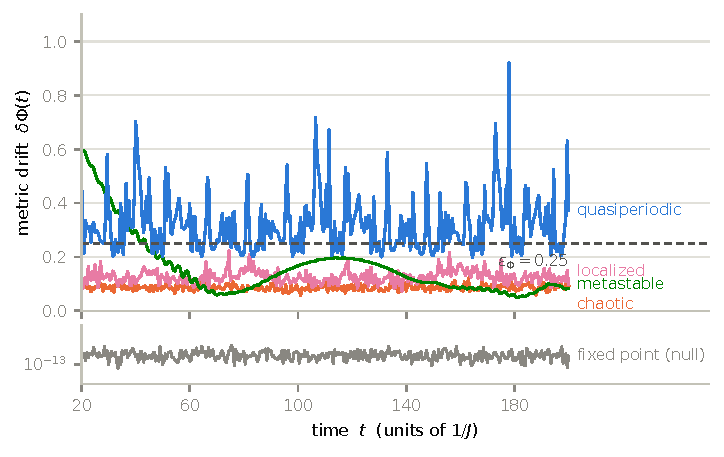
\includegraphics[width=\linewidth]{fig2_drift.pdf}
\caption{Metric drift $\delta\Phi(t)$ for representative runs
($N=10$). The chaotic metric is stationary under the preregistered
threshold while the quasiperiodic metric oscillates far above it; the
metastable class shows its slow coherent wave; the localized run sits
near the threshold (the class straddles it, 80/100 stationary at
$N=12$). Bottom strip: the frozen null at machine precision. Ensemble
verdicts are given in the text.}
\label{fig:drift}
\end{figure}

At the calibrated threshold $\ephi = 0.25$, the chaotic and scrambling
ensembles are metric-stationary in every run (20/20 at each size; max
window drift $0.09$--$0.21$) while their motion witnesses read near
maximum: $\Xi \geq 0.96$, recurrence mean $\approx 1 - 1/D$, and Bohr
participation ratios in the hundreds to thousands. The driven track is
the sharpest instance: at drive imperfection $\varepsilon = 0.03$, all
100 runs are metric-stationary while the subharmonic witness reads
$0.939$ --- a locked period-doubled magnetization response over a
frozen mutual-information metric. At the other extreme, the
quasiperiodic and metastable classes have genuinely moving metrics (max
drift $0.53$--$1.61$; no run stationary), the integrable regime
likewise ($0.35$--$0.64$), and the fixed point is stationary to machine
precision ($2\times10^{-13}$) with every witness silent --- the null
behaving as a null. The localized regime straddles the threshold
(80/100 stationary at $N=12$, drift $0.14$--$0.34$) and is treated as a
boundary case throughout.

Two honesty notes frame everything that follows. First, for the
chaotic classes, metric stationarity over motion is \emph{expected}:
the metric is built from two-site observables, and the equilibration of
local observables in quenched chaotic systems is standard physics. The
existence table is the setup, not the result. Second, none of these
verdicts is an artifact of the weight floor in the metric construction:
the above-floor drift diagnostic tracks the full-graph drift in every
class, and the mean graphs have no floor-dominated links.

\section{Results II: the witness discipline at work}\label{sec:witness}

This section reports the study's methodological core: what the
preregistered witness requirements did when the data pushed back. We
present it as a dual record --- the original registration failed; the
ratified repair passed on fresh seeds --- because both halves are
results (Fig.~\ref{fig:witnesses}).

\begin{figure*}[t]
\centering
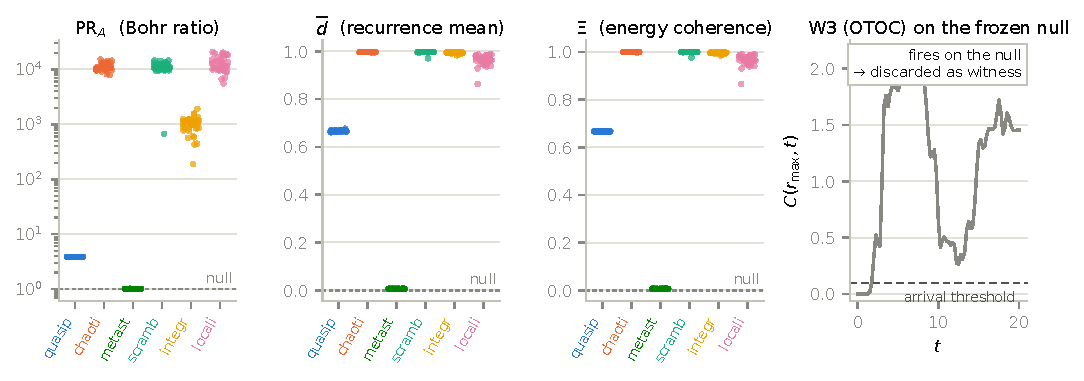
\includegraphics[width=\textwidth]{fig3_witnesses.pdf}
\caption{The final witness battery (fresh seeds, $n=40$, $N=12$; per-run
values, one dot per run). Dashed lines: the frozen null's exact values.
All three statistics are null-silent; class separation is visible
directly. Right panel: the registered witness W3 (OTOC) evaluated on
the frozen null --- it crosses its own arrival threshold at $t^*=1.5$
and saturates near $1.1$--$1.5$, firing on a state that does not move;
under the preregistered null-silence clause it was discarded from the
criterion.}
\label{fig:witnesses}
\end{figure*}

\textbf{The OTOC is not a witness of motion.} The null-silence
requirement (Sec.~\ref{sec:witnessdef}) demands that a witness vanish
on the frozen class-(i) state. The out-of-time-order correlator fails:
on the gapped ground state it reaches the arrival threshold at
$t^*=1.5$ and saturates at $C \approx 1.11$. Nothing is wrong with the
OTOC as physics --- it certifies operator spreading, which a frozen
state supports --- but that is precisely why it cannot certify that a
\emph{state} is moving. The preregistered discard clause executed,
removing both OTOC statistics from the class-separation criterion.

\textbf{The discard had teeth.} With the OTOC gone, the original
battery left exactly one class pair under-witnessed: scrambling vs.\
localized separated on $\Xi$ alone (AUC $0.985$/$0.990$ at the two
sizes), with the Bohr participation ratio degrading with size ($0.89
\to 0.56$) and the registered recurrence statistic --- the window
\emph{minimum} --- landing at $0.71$/$0.945$. Criterion~(a), as
originally registered, therefore \textbf{fails}. The counterfactual is
recorded: had the OTOC been retained, its arrival time separates that
pair at AUC $1.0$ (localized fronts never arrive; scrambling fronts
arrive at $t \approx 2$). The failure is single-cause, and it is a
finding about witness design: the natural scrambling/localization
discriminator is not null-silent, and the null-silent battery we
registered was one statistic short.

\textbf{The repair, and what fresh seeds taught us.} The reformalized
battery replaces the recurrence minimum --- structurally uninformative
for slow classes, since a slowly rotating state revisits its reference
--- with the recurrence \emph{mean}, which is null-silent by
construction and class-resolving in practice. On the data that
motivated the redesign, all 18 pair-size checks passed; we labeled that
table validation, not confirmation, and re-adjudicated on fresh
committed seeds. At the registered ensemble size ($n=20$) the fresh
seeds \textbf{failed} a different pair --- scrambling vs.\ integrable
at $N=10$, all three statistics between $0.85$ and $0.93$ --- while
passing at $N=12$. The diagnosis is statistical, not physical: a sharp
AUC threshold of $0.95$ estimated from 20-vs-20 samples carries a
standard error of $0.05$--$0.08$, so near-threshold verdicts are
seed-lotteries. Doubling the ensembles ($n=40$, fresh seeds again)
stabilized every margin: \textbf{all 18 pair-size checks pass}, the
previously marginal pair at $0.952$--$0.979$, and the repaired pair at
$0.987$--$0.992$ (the Bohr ratio for scrambling vs.\ localized remains
honestly weak, $0.59$ at $N=12$ --- two statistics carry the pair, as
the criterion requires). A descriptive third size ($N=14$, computed
from eigenbasis coefficients alone) confirms the monotone trend: all
three statistics $\geq 0.976$.

To keep the epistemic status of each stage unambiguous, Table~\ref
{tab:stages} separates them explicitly; only the first row carries the
original registration's status, and the final verdict is
\emph{pre-committed} (fresh seeds, outcome accepted in advance either
way, under ratified amendments) rather than preregistered.

\begin{table}[t]
\centering\footnotesize
\begin{tabular}{@{}p{3.15cm}p{1.9cm}p{2.15cm}@{}}
\toprule
stage & status & outcome \\
\midrule
original battery, registered seeds & registered & (a) FAILS \\
reformalized battery, original seeds & exploratory & 18/18 (validation
only) \\
reformalized, fresh seeds, $n{=}20$ & pre-committed & FAILS (marginal
pair) \\
reformalized, fresh seeds, $n{=}40$ & pre-committed & \textbf{PASSES
18/18 (final)} \\
\bottomrule
\end{tabular}
\caption{Stages of the class-separation criterion. Amendments between
stages are dated in Appendix~\ref{app:log}.}
\label{tab:stages}
\end{table}

The two methodological claims we take from this: null-silence is a
nontrivial filter that separates state-motion witnesses from
operator-spreading diagnostics; and sharp-threshold criteria on small
ensembles must be fresh-seeded and, near the threshold,
power-stabilized --- our original-seed validation table would have
over-claimed.

\section{Results III: class-resolved robustness and the dephasing sign
structure}\label{sec:robust}

The robustness criterion asks whether metric stationarity responds to
perturbation differently in different dynamical classes. Under local
dephasing at the calibrated rate $\gamma = 0.01$, it does, with a sign
structure that is the study's most striking single measurement
(Fig.~\ref{fig:gamma}).

\begin{figure}[t]
\centering
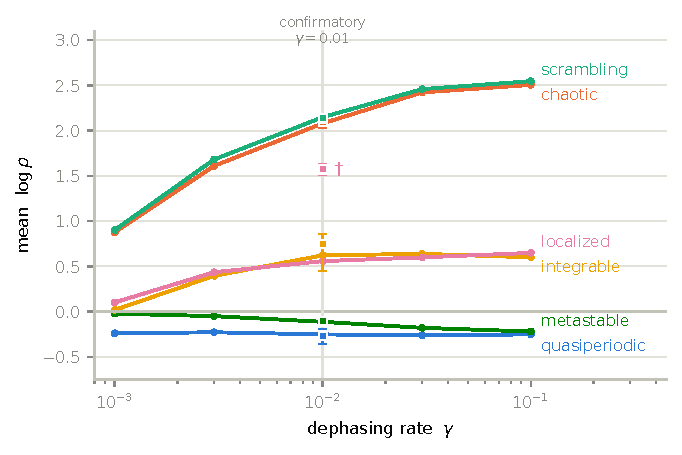
\includegraphics[width=\linewidth]{fig4_gamma.pdf}
\caption{Dephasing response by class: mean $\logr$ versus rate
$\gamma$ (descriptive sweep, curves; first 10 manifest runs per class,
N\'eel-primary for the localized regime). Squares with intervals: the
confirmatory single-$\gamma$ ensemble means with BCa 95\% CIs.
($\dagger$: the confirmatory localized ensemble uses 5 initial states
per realization and reads higher than the N\'eel-primary sweep --- an
ensemble-composition difference, not a discrepancy.) The sign
structure --- negative for coherence-carried classes, strongly positive
for chaotic ones --- is stable over two decades and never reorders.}
\label{fig:gamma}
\end{figure}

The mean log drift ratios, replicated at two sizes with disjoint
confidence intervals and consistent direction: chaotic and scrambling
$+2.1$ to $+2.2$ (noise strongly destabilizes their stationary
metrics), localized $+1.5$, integrable $+0.75$ --- and the
coherence-carried classes \emph{negative}: metastable
$-0.09$/$-0.11$, quasiperiodic $-0.27$. Weak dephasing makes the
quasiperiodic metric \emph{more} stationary than its own unperturbed
dynamics: the noise damps the coherences whose beating carries the
metric's oscillation, pinning $D(t)$ to its time average. Every
pairwise contrast required by the registered criterion clears the
$\ln 1.5$ threshold in both tracks at both sizes; the class ordering
(chaotic $\approx$ scrambling $>$ localized $>$ integrable $>$
metastable $\gtrsim$ quasiperiodic, the last two negative) is the
pilot's ordering, confirmed at scale.

A descriptive strength sweep shows the sign structure is a regime, not
a point: across two decades $\gamma \in [10^{-3}, 10^{-1}]$ the
quasiperiodic response is flat at $\approx -0.25$, the metastable
response strengthens monotonically ($-0.02 \to -0.22$), the
chaotic-class response rises and saturates ($+0.9 \to +2.5$), and the
ordering never reorders. The mechanism is standard open-system physics
--- decoherence damping of coherence-carried oscillations, the
weak-rate side of the Zeno family \cite{SRC059} --- and we claim none
of it as new. The class-resolved \emph{geometric} reading --- noise as
a stabilizer of moving information metrics and a destabilizer of
chaotic ones, with the sign tracking the dynamical class --- is, to the
extent of our survey \cite{SRC060,SRC061,SRC062,SRC063}, unreported;
we state this conditionally and note the survey was not systematic.

The other two protocols are clean nulls at the registered strengths:
the local quench leaves every dynamical class's drift ratio at
$|\overline{\logr}| \leq 0.07$, and two-site loss reads $0.07$--$0.25$
everywhere. (The fixed point's large quench ratio, $+4.4$, is
floor-referenced --- its unperturbed drift is exactly zero --- and
carries no class information; instrument note in
Appendix~\ref{app:stats}.) All robustness statements are statements at
the calibrated strengths and, per the sweep, within the probed regime
--- not strength-independent class properties.

\section{Results IV: the motionless-comparator search --- existence
versus naturalness}\label{sec:comparator}

The sharpest form of the maintained-vs-instantiated question is:
\emph{does there exist a motionless state carrying the same
time-averaged metric --- and if so, how complicated must it be?} An
important caveat frames this whole section: for the classes whose
metric is genuinely moving (quasiperiodic, metastable, integrable),
the object under discussion is the \emph{time-averaged} metric
$\bar D$, which is a stationary summary by construction; only for the
metric-stationary classes is $\bar D$ also the metric one would
observe. This section reports the search, including the three
corrections that shaped it --- two forced by our own audits, one by an
external pre-submission review (Fig.~\ref{fig:comparator}).

\begin{figure*}[t]
\centering
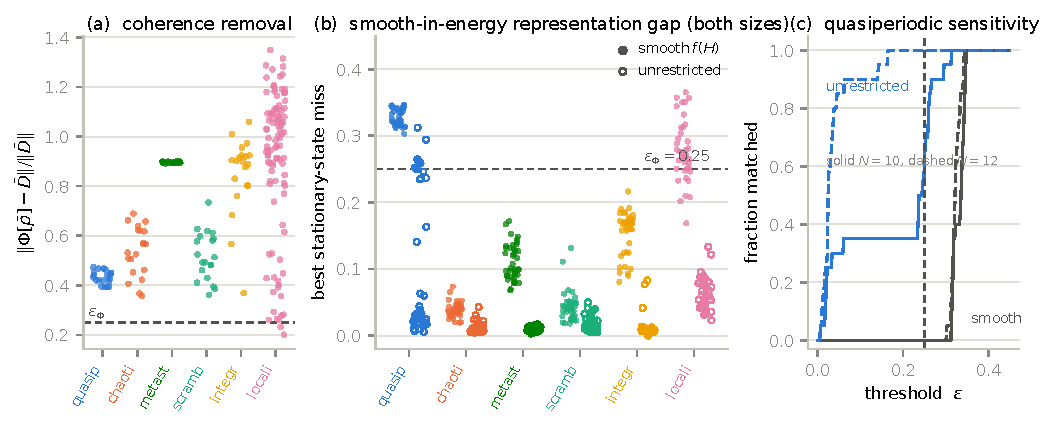
\includegraphics[width=\textwidth]{fig5_comparator.pdf}
\caption{(a) The coherence-removal measurement: projecting the state
onto its diagonal ensemble mid-window moves the metric by 43--90\% of
$\lVert\bar D\rVert$ in every class --- removing the motion changes
the metric. (b) The naturalness gap: best achievable miss
$\lVert\Phi[\sigma]-\bar D\rVert/\lVert\bar D\rVert$ per run, both
sizes pooled, for smooth-$f(H)$ stationary ensembles (filled; $\leq
24$ parameters) versus unrestricted diagonal-population optimization
(rings; $2^N$ parameters). Every class is matchable by the
unrestricted search; only the quasiperiodic class requires it. (c)
Threshold sensitivity for the quasiperiodic class: fraction of runs
matched versus threshold, per search family and size; the registered
$\ephi = 0.25$ (vertical line) sits in the steep region of the
unrestricted $N=10$ curve, so counts at that threshold are
sensitive --- the smooth/unrestricted gap is not.}
\label{fig:comparator}
\end{figure*}

\textbf{The canonical comparator is not matched.} The diagonal ensemble
$\bar\rho$ --- the motionless state with the run's exact time-averaged
two-site reduced density matrices --- was registered as metric-matched
by construction. It is not: mutual information is nonlinear in the
reduced density matrices, and $\Phi[\bar\rho]$ sits $43$--$90\%$ of
$\lVert\bar D\rVert$ away from the run mean, depending on class.
Relatedly, our first robustness comparison against $\bar\rho$ produced
a large ``the comparator is more fragile'' differential that an
adversarial re-analysis exposed as a floored-denominator artifact (the
comparator has no baseline drift to compare against; its absolute
perturbed response is in fact \emph{smaller}). Both corrections are
dated in the study record; what survives them is stronger than what
they replaced.

\textbf{The coherence-removal measurement.} Projecting onto $\bar\rho$
mid-window moves the metric by $43$--$90\%$ of $\lVert\bar D\rVert$
(chaotic $0.54$, scrambling $0.52$, integrable $0.85$, metastable
$0.90$, localized $0.90$, quasiperiodic $0.43$). Removing the motion
does not freeze the metric in place; it changes the metric. For the
metric-stationary classes this registers as a drift increase with
disjoint confidence intervals.

\textbf{The three-stage search.} Stationarity means $[\sigma, H]=0$,
so we optimized over populations on the energy eigenbasis, in three
stages of increasing freedom, over full ensembles at both criterion
sizes: (i) three natural families (thermal at both temperature signs,
depolarized diagonal ensemble, Gaussian microcanonical; $\leq 2$
parameters each); (ii) a smooth-$f(H)$ family (log-populations
parameterized by up to 24 Chebyshev coefficients in the scaled energy,
multi-start); (iii) --- prompted by an external pre-submission review
that correctly observed stage (ii) is not all stationary states ---
an \emph{unrestricted} optimization over all $2^N$ populations
(softmax parameterization, analytic gradient through the entropies and
shortest paths, gradient verified against finite differences,
multi-start). Two earlier over-claims are part of the record: the
family-only stage wrongly suggested metastable and integrable were
unmatchable (corrected at stage ii), and stage (ii) wrongly suggested
the quasiperiodic class was categorically unmatched (corrected at
stage iii).

The final result is a \textbf{complexity split, not an existence
split}. Under the unrestricted search, \emph{every} class is matchable
within $\ephi$ at $N=12$ --- quasiperiodic included (20/20, median
miss $0.025$); at $N=10$ the quasiperiodic class straddles the
threshold (12/20, median $0.241$) while every other class matches in
every run (medians $0.008$--$0.066$). This is partly a
parameter-counting effect: the number of free populations grows as
$2^N$ while the target has only $N(N-1)/2$ entries, so unrestricted
matchability becomes generic with size. The size-robust,
class-resolved quantity is the cost of the match. Within
smooth-$f(H)$ ensembles --- whose parameter count does not grow with
dimension --- chaotic and scrambling metrics are matched almost
exactly in every run (median $0.035$--$0.046$; a Gaussian
microcanonical window suffices, as eigenstate thermalization would
suggest), metastable ($0.09$--$0.13$) and integrable ($0.16$--$0.17$)
follow, localized is marginal (median $\approx 0.27$), and \textbf{the
quasiperiodic time-averaged metric is unmatched in 0 of 80 runs
(median $0.31$--$0.34$)}, robustly across mode numbers $m = 3, 4, 5$.
The quasiperiodic $\bar D$ is reproducible only by fine-tuned
population vectors with dimension-scaling parameter counts: the
class discriminator is the \emph{description complexity of the
cheapest motionless impostor}, and Fig.~\ref{fig:comparator}(c) shows
the gap between the smooth and unrestricted searches is insensitive to
the threshold choice even where the counts at $\ephi$ are not.

Two independent instruments still single out the same class, in this
corrected sense: the quasiperiodic metric is the only one with no
\emph{natural} (smooth, low-parameter) motionless double, and the only
one that weak noise \emph{stabilizes} (Sec.~\ref{sec:robust}). Whether
some principled measure of stationary-state complexity makes the
naturalness gap precise --- and whether it survives larger systems,
where parameter counting increasingly favours fine-tuned matches ---
we pose as the open question this study leaves sharpest. Conversely,
the chaotic classes' stationary metrics are straightforwardly
compatible-with their motion: the simplest thermal impostor carries
the same structure, while the robustness signature of
Sec.~\ref{sec:robust} still distinguishes the classes dynamically.

\section{Results V: the driven regime}\label{sec:driven}

The driven track --- a kicked-Ising protocol in its rigid subharmonic
(DTC-like) regime \cite{SRC043,SRC044,SRC054} --- supplies the study's
cleanest stationary-with-witness regime and its most instructive
compatible-with verdict (Fig.~\ref{fig:driven}). We say ``DTC-like''
deliberately: at $N \leq 14$ with 20 disorder realizations we observe
locked subharmonic response and a rigidity curve consistent with the
discrete-time-crystal phase, but we perform no size or lifetime
scaling and make no phase claim \cite{SRC054}.

\begin{figure*}[t]
\centering
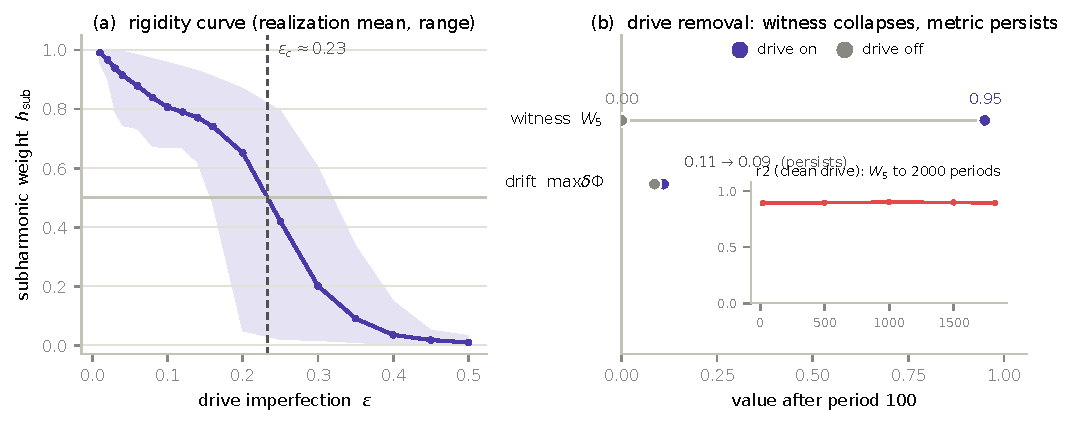
\includegraphics[width=\textwidth]{fig6_driven.pdf}
\caption{(a) The full rigidity curve of the driven track: subharmonic
weight $h_{\rm sub}$ versus drive imperfection (realization mean and
range, seed-paired across $\varepsilon$), crossing $1/2$ at
$\varepsilon_c \approx 0.23$ (interpolated). (b) The drive-removal test
at $\varepsilon=0.03$: removing the kicks collapses the subharmonic
witness while the metric drift persists essentially unchanged ---
localization, not the drive, holds this metric. Inset: the clean
interacting comparator (r2) does not thermalize on any probed horizon;
its subharmonic weight is undiminished at 2000 periods.}
\label{fig:driven}
\end{figure*}

At $\varepsilon = 0.03$, deep in the rigid regime, all 100 runs are
metric-stationary while the subharmonic witness reads $0.939$: a
period-doubled magnetization response, locked across 20 disorder
realizations, above a mutual-information metric that does not move.
Stationarity degrades with drive imperfection (88/100 at $\varepsilon =
0.06$, 52/100 at $0.10$), tracking the witness. The rigidity curve is
measured over its full range: the subharmonic weight holds above
$0.65$ through $\varepsilon = 0.20$, crosses $1/2$ at $\varepsilon_c
\approx 0.23$ at our drive parameters, and collapses by $\varepsilon
\approx 0.45$ --- a complete critical-strength measurement for this
realization of the protocol of Refs.~\cite{SRC043,SRC044}.

The drive-removal test resolves the maintained-vs-instantiated
question for this regime, and resolves it \emph{against} the drive:
removing the kicks at mid-window collapses the witness
($0.95 \to 0.00$) while the metric's stationarity persists and
slightly improves (mean post-window drift $0.110 \to 0.086$). The frozen-in disorder, not the drive, holds this
metric --- the witnessed subharmonic motion is compatible with the
stationary structure, not required by it. We registered this as an open
question with exactly this outcome listed as reportable, and report it
accordingly. Consistently, the perturbation protocols at the calibrated
strengths barely move the DTC-like regime's metric ($\overline{\logr} =
0.01$--$0.19$).

The comparator regimes behave asymmetrically, and honestly. Without
interactions (r1), the subharmonic peak is destroyed at $\varepsilon =
0.03$ ($0.13$) --- the fine-tuned control fails as expected, certifying
that interactions produce the rigidity. Without disorder (r2), however,
the clean interacting drive does \emph{not} thermalize on any horizon
we probed: its subharmonic response persists undiminished
($0.89$--$0.90$) to 2000 periods. At small $\varepsilon$ the r2 regime
is not a usable thermalizing control, and the discriminating comparator
burden falls entirely on r1 --- a comparator-scope finding we report
rather than bury.

\section{Scope walls and limitations}\label{sec:scope}

\textbf{The metric belongs to the factorization.} Everything here is
computed on the natural site partition, and the dependence on that
choice is not small and not uniform: under fixed nonlocal two-site
frame changes, the metric moves by a class-dependent amount --- mean
relative change $0.11$ (chaotic), $0.15$ (scrambling), $0.20$
(localized), $0.22$ (integrable), $0.42$ (quasiperiodic), $0.53$
(metastable, maximum observed $0.82$). The coherence-carried classes
--- including the survivor class of Sec.~\ref{sec:comparator} --- have
the most frame-dependent metrics. This does not undermine the
within-frame comparisons (every matchability and robustness statement
compares objects in the same partition, which transforms both sides
together), but it bounds the interpretation: these are properties of
the metric-on-a-factorization, not of the state alone. Notably,
strictly local (single-site) frame changes leave the metric invariant
to machine precision --- the dependence lives entirely at the partition
level, which is where the construction's own authors located their
caveat \cite{SRC049}.

\textbf{Finite size, finite family, finite search.} Criterion verdicts
are established at $N \in \{10, 12\}$ with a descriptive $N=14$ point;
the quasiperiodic construction is exhaustively unsatisfiable at $N=8$
(0/56 candidate mode triples), which is a warning about small-size
instantiations of incommensurability generally. The stationarity
threshold $\ephi = 0.25$ is calibrated to this construction's
finite-size noise floor and has no significance beyond it. The
comparator search spans stationary states that are smooth functions of
$H$; fine-tuned non-smooth populations are outside it, and the
unmatchability result is bounded accordingly. The localized regime
straddles the stationarity threshold (80/100) and we have kept it out
of every headline count. Robustness statements hold at the calibrated
strengths and within the swept regime ($\gamma \in [10^{-3},
10^{-1}]$). All clocks are external laboratory clocks; nothing here
addresses systems that must supply their own.

\section{Discussion and outlook}\label{sec:discussion}

What the study delivers is not a mechanism but an instrument, and a
measured answer narrower than the question in our title. Is the
emergent metric motion-borne? Not in the existential sense we
initially hoped to establish: every class's time-averaged metric,
including the quasiperiodic one, is carried by \emph{some} stationary
state once fine-tuned, dimension-scaling population vectors are
allowed. What the measurements do establish is threefold: time
averaging and metric construction do not commute (the canonical
motionless partner misses by 43--90\%); the cost of a motionless
reproduction is sharply class-resolved, with thermalizing classes
matched by three-parameter thermal windows and the quasiperiodic class
by nothing smooth at all; and weak noise stabilizes exactly the class
that resists natural stationary description. ``Motion-borne'' survives
as a motivating question and as an open conjecture about
\emph{natural} stationary descriptions --- not as a demonstrated
existential conclusion.

The sharpest open question the data leaves is the naturalness gap
itself: is there a principled complexity measure on stationary states
(parameter count is a crude proxy) under which the quasiperiodic
time-averaged metric is provably expensive --- and does the gap
survive larger systems, where parameter counting increasingly favours
fine-tuned matches? A second question follows the sign structure: is
there a form of robustness that \emph{recurrent} or quasiperiodic
dynamics provides and fixed points cannot? The coincidence reported
here --- the hardest-to-match class is the one noise defends --- is
the evidence such a mechanism would leave, and the driven track
supplies a controlled arena in which to look (with the caution of
Sec.~\ref{sec:driven}: the most spectacular witnessed motion in this
study turned out \emph{not} to hold its metric).

The test template itself is not specific to spin chains. Any system
with a computable structural functional over a dynamical substrate
admits the same three probes: certify the motion with null-silent
witnesses, remove the coherence that carries it, and search honestly
for a motionless impostor --- reporting the impostor's complexity, not
just its existence. Candidate applications suggest themselves wherever
stable emergent structure rides on flux --- resting-state functional
connectivity over neural dynamics, metabolic network structure over
flux-carrying steady states, stability of ecological or market
structure over turnover --- and we offer the template for these
settings as a proposal only: nothing beyond spin chains has been
demonstrated here. The distinction the test operationalizes ---
structure that merely exists versus structure that is actively kept in
existence --- is, of course, much older than physics; we make no
attempt to engage that literature here.

On the methods side, we draw two conclusions we believe generalize.
Null tests for witnesses are cheap and clarifying --- the OTOC episode
suggests that diagnostics informally credited with certifying
``dynamics'' deserve routine auditing against frozen states, if only
to fix which kind of dynamics they certify. And a registered design
with committed seeds changed the outcome of this study five times ---
four corrections from our own audit mechanisms and one from external
review; the amendment log (Appendix~\ref{app:log}) is our answer to
the question of what such discipline buys in a purely computational
setting.

The obvious open front is scale and covariance: whether any version of
this question can be asked of structures that deserve the word
``geometry'' with fewer scare quotes --- partition-covariant
functionals, larger systems, internally clocked dynamics --- remains
exactly as open as it was, and none of the present results shortens
that road. What they do establish is that the road's first step is
measurable: already in twelve qubits, one can ask what a structure's
cheapest motionless impostor costs, and get a class-resolved answer.

\paragraph{Acknowledgements.} The numerical study --- implementation,
execution, analysis, and the adversarial companion --- was carried out
with Claude (Anthropic) as AI research assistant, operating under the
preregistration and shared-substrate protocol whose record forms
Appendix~\ref{app:log}. The programme's initiating knowledge base was
drafted in collaboration with OpenAI's ChatGPT. An external
pre-submission review prompted the unrestricted comparator analysis
and several framing corrections reported here. All rulings, decisions,
and the final text are the author's responsibility.

\paragraph{Funding.} This work received no external funding; it was
carried out in the author's free time, for the joy of it.

\paragraph{Data and code availability.} The full study record ---
specification, seed manifests, amendment log, evidence packets, session
logs, analysis code, and all run outputs --- is available in the public
repository \url{https://github.com/olegroshka/ideg}, pinned at the
submission tag (\texttt{paper-v1}).

\appendix

\section{Numerics}\label{app:numerics}

\paragraph{Models and distributions.} Track-A/C Hamiltonians and
parameters are fully specified in Table~\ref{tab:classes} and
Sec.~\ref{sec:family}; disorder draws are $h_i \sim U[-W, W]$ with
$W=8$ for the localized regime and $\delta g_i \sim U[-0.01, 0.01]$
for the metastable dressings. The driven track evolves by the Floquet
unitary $U_F = e^{-iH_2 t_2}\, e^{-iH_1 t_1}$ with $t_1 = t_2 = 1$,
$H_1 = \tfrac{\pi}{2}(1-\varepsilon)\sum_i \sigma^y_i$ and
$H_2 = \sum_i J_i\,\sigma^z_i\sigma^z_{i+1} + \sum_i h_i\sigma^z_i$,
$J_i \sim U[0.05, 0.15]\pi$, $h_i \sim U[0, \pi]$ (r1 sets $J_i = 0$;
r2 sets $h_i = 0$); disorder and initial states are seed-paired across
$\varepsilon$ and regimes.

\paragraph{Dephasing channel.} The perturbation protocol applies local
$\sigma^z$ dephasing at rate $\gamma$: Lindblad generator
$\mathcal{D}[\rho] = \gamma\sum_i (\sigma^z_i \rho\, \sigma^z_i -
\rho)$, implemented by Trotter splitting (step $0.5$) of the exact
unitary and the exact damping mask $e^{-2\gamma\,\Delta t\, d_H(a,b)}$
on the computational-basis coherences, $d_H$ the Hamming distance ---
exact for the commuting pure-dephasing part, splitting error
$O(\Delta t^2)$.

\paragraph{Comparator optimization.} The stationary search minimizes
$\lVert\Phi[\sigma(p)] - \bar D\rVert_F / \lVert\bar D\rVert_F$ over
eigenbasis populations $p$. Stages: fixed families (grids over
$\beta$, depolarization $\lambda$, and Gaussian window $(E_0,
\sigma_E)$); smooth $f(H)$ ($\log p = \sum_{k<K}
c_k T_k(\tilde E)$, $K \leq 24$, Powell, multi-start, $\leq 800$
evaluations per start); unrestricted ($p = \mathrm{softmax}(\theta)$,
$\theta \in \mathbb{R}^{2^N}$, L-BFGS-B with the analytic gradient
assembled from $\partial S/\partial p_n = -\mathrm{tr}[R_n(\ln\rho +
1)]$ per reduced density matrix, $\partial w/\partial x = -1/x$ off
the weight floor, and shortest-path edge subgradients from
predecessor-tracked Floyd--Warshall; five starts including the best
smooth solution; gradient verified against finite differences,
relative deviation $1.7\times10^{-3}$, dominated by path-tie
subgradients). Convergence: L-BFGS-B to $\lVert g\rVert < 10^{-8}$ or
400 iterations; multi-start scatter across the five starts is small
compared to the class gaps reported.

\paragraph{Diagonalization and evolution.}
Exact diagonalization throughout (dense to $N=14$, dimension 16384);
pure-state evolution via eigendecomposition, density-matrix evolution
for the dephasing protocol via Trotter splitting of the unitary and the
exact per-step damping mask (step $0.5$), $N \leq 10$. State-norm drift
across all unitary runs $< 4\times10^{-15}$; trace drift of dephased
runs recorded per run at the same scale. Python~3.11 / NumPy~2.3 /
SciPy~1.15; every random draw seeded from committed manifests; total
compute across pilot, confirmatory, adversarial, and hardening
campaigns of order a machine-day on a 24-core workstation. The $N=14$
witness point uses the identity $|\langle\psi(t_0)|\psi(t)\rangle|^2 =
|\sum_n p_n e^{-iE_n(t-t_0)}|^2$, so recurrence statistics require only
eigenbasis coefficients. The comparator search precomputes
per-eigenstate two-site reduced density matrices, making each candidate
stationary state's metric a population-weighted sum evaluable in
milliseconds at any dimension.

\section{Statistics}\label{app:stats}

Class separation: exact Mann--Whitney AUC, symmetrized $\max(A, 1-A)$
since direction is not registered; threshold $0.95$; $\geq 2$
statistics per pair; two sizes; singleton classes (the fixed point) by
exact-value exclusion (the ensemble range must exclude the
deterministic value). Robustness: mean log drift ratio per class, BCa
bootstrap (1000 resamples, 95\%), disjoint intervals plus $|\Delta| >
\ln 1.5$, replicated with consistent direction; disordered ensembles
resampled at the realization level. Seed sensitivity: at $n=20$-vs-20
the AUC standard error near $A \approx 0.9$ is $0.05$--$0.08$, so
verdicts within one standard error of threshold are lotteries ---
measured directly here when fresh seeds flipped a marginal pair
(Sec.~\ref{sec:witness}); $n = 40$ halves the standard error and
stabilized every margin. Size trend for the marginal pair (AUC at $N =
10 \to 12 \to 14$): Bohr ratio $0.979 \to 0.979 \to 1.000$; recurrence
mean $0.952 \to 0.975 \to 0.976$; energy coherence $0.956 \to 0.975 \to
0.976$. Instrument notes: the log-ratio floor ($10^{-3}$) makes
exactly-stationary objects read $\logr \approx
\log(\delta\Phi_{\rm pert}/10^{-3})$ --- class-(i) quench values are
floor-referenced and excluded from class inference; the metric's
$-\ln x$ weight cap amplifies machine-epsilon mutual-information jitter
by up to $x_{\min}^{-1}=10^6$, setting an irreducible $\sim 10^{-9}$
numerical floor on metric-space identity checks for near-product
states.

\section{The amendment log}\label{app:log}

The complete dated record of every post-registration change, each with
its reason and repository commit; no entry alters data already taken.

\begin{table*}[t]
\centering\footnotesize
\begin{tabular}{@{}p{1.25cm}p{9.55cm}p{2.55cm}@{}}
\toprule
date & entry & commit \\
\midrule
08-11 & Spec registered; threshold review (Am.~1): criterion-(b)
instrument $\to$ log drift ratio + calibration pilot &
\texttt{24eaa858ec60}\newline\texttt{7e40011d56c8} \\
08-11 & Am.~2 (pre-run): integrable certificate Poisson $\to$
free-spectrum reconstruction (mis-specification measured: free chain) &
\texttt{602658b1b96c} \\
08-11 & Am.~3 (pilot, owner-ruled): $\ephi\ 0.05 \to 0.25$ (below
measured noise floor); confirmatory $\lambda=0.1$, $\gamma=0.01$ &
\texttt{5db69bade460} \\
08-12 & Instrument survey: KEEP log-ratio (no change; dated entry) &
\texttt{27ada59e697c} \\
08-12 & Confirmatory manifest committed pre-execution; survey window
closed at first run & \texttt{b91ad54da91f} \\
08-12 & Addendum~1: quasiperiodic construction unsatisfiable at $N=8$
(0/56, exhaustive) $\to$ criterion sizes (10, 12) &
\texttt{a76db0e67e09} \\
08-12/13 & Confirmatory executed: W3 fires on null $\to$ discarded;
(a) fails as registered; (b) holds; verdicts of record &
\texttt{fbe324f38f34} \\
08-13 & Adversarial companion: fragility-direction retraction (floored
denominator); comparator matching assumption refuted &
\texttt{33fdd6287776} \\
08-13 & Am.~4 (ratified): battery $\to$ $\{\mathrm{PR}_A, \overline{d},
\Xi\}$; W3 descriptive; fresh-seed re-adjudication required &
\texttt{9030c0ebdab6} \\
08-13 & Fresh seeds $n=20$: FAIL on a different, threshold-marginal
pair (seed lottery measured) & \texttt{5efaa7309c56} \\
08-13 & Am.~5 (ratified): $n = 40$, final verdict accepted either way
$\to$ (a) HOLDS 18/18 & \texttt{3e7c0a787a09} \\
08-13 & Hardened comparator search corrects family-only over-claim:
single-survivor result & \texttt{67dda68970b1} \\
08-13 & Descriptive hardening sweep: $\varepsilon_c$, 2000-period
comparator, $\gamma$-grid, partition distribution, $N=14$ &
\texttt{9ce17dec803c} \\
08-14 & External pre-submission review received; core criticisms
accepted (time-average framing; search-space bound) &
--- \\
08-14/15 & Unrestricted comparator optimization (review-prompted):
every class matchable; smooth-vs-unrestricted naturalness gap replaces
the single-survivor claim & \texttt{075eb96},
\texttt{2978713} \\
08-15 & Major revision: non-commutation thesis; coherence-removal /
drive-removal renaming; tempered OTOC framing; DTC-like wording;
stages table; self-contained numerics & (this build) \\
\bottomrule
\end{tabular}
\caption{The amendment log (12-character commit identifiers in the
public repository).}
\label{tab:log}
\end{table*}

\section{Invariance battery}\label{app:battery}

Every witness statistic and the metric were checked under: global
phase; consistent local basis change (state, Hamiltonian, and operators
together); local basis change of the state alone; and site reflection.
Witness statistics and mutual-information matrices are identical within
$10^{-10}$ in all mandatory items across every class and size (the
participation ratio judged relative to its own magnitude, which reaches
$10^5$--$10^6$ at $N=12$). Metric-space deviations carry the
cap-amplified numerical floor described in Appendix~\ref{app:stats} and
are reported, not thresholded. The state-only local change leaves the
metric invariant to machine precision --- single-site entropies are
local-frame invariant --- which localizes all factorization dependence
at the partition level; the partition probe of Sec.~\ref{sec:scope}
(fixed random entangling two-site frames on three disjoint pairs,
24--72 samples per class) is the quantitative version.

\section{Driven-track implementation notes}\label{app:tb}

Disorder realizations and initial states are seed-paired across drive
strengths and comparator regimes (identical couplings and fields at
equal seed), so rigidity curves and regime contrasts are paired
comparisons. The subharmonic weight is computed on an even number of
stroboscopic periods so the period-doubled line is the exact Nyquist
bin. Drive removal evolves under the interaction Hamiltonian alone in lab
time, sampled at the same period boundaries (drive removed, clock
kept). The dephasing protocol applies the exact per-period damping mask
with the rate stated in lab-time units ($T_{\rm period} = 2$).

\bibliographystyle{unsrt}
\bibliography{references}

\end{document}
